\subsection{Implementation and deployment}
\label{sec:deployment}

%\begin{figure}[t]
%  \centering
%  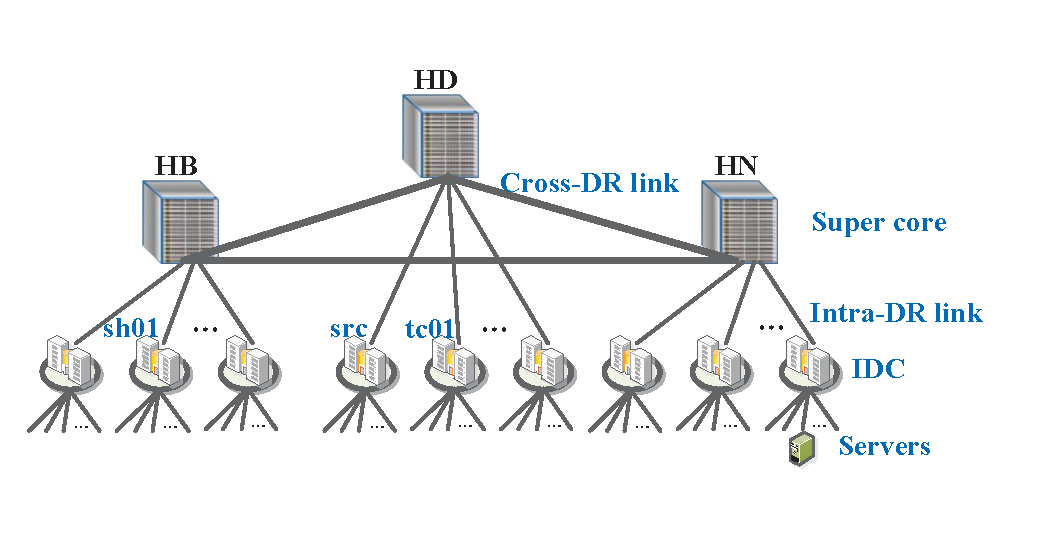
\includegraphics[width=3in]{images/Testbed_v2.eps}
%  \tightcaption{The abstract topology of our intra-net WAN.}
%  \label{fig:topology}
%\vspace{-0.1in}
%\end{figure}
%\vspace{-15pt}

We have deployed \name on \company's DCs, which consist of 67 geo-distributed servers in 10 DCs. Evaluations in the next section are based on this deployment. %The topology is shown as Fig. \ref{fig:topology}.

\name is implemented with 3621 lines of golang code \cite{golang}, and it can be fully integrated in \company's DCs. The three duplications of the controller are implemented on three different geo-located servers. The data plane (bulk data transmissions) between controller and agents adopts TCP, and the control plane (decision messages) adopts HTTP. For specific transmissions, \name uses \texttt{wget} to make data transfer and sets particular \texttt{wget} options to enforce bandwidth. \jc{which option?}

This implementation makes no specific requirements on applications, and any application prepares to distribute bulk data just needs to follow three steps: first, register on \name, initiate the basic information about source DC, destination DCs, all end servers and the bulk data; second, install agents on the involved end servers; third, assign the start time of bulk data transmission. Then \name will start the data distribution at the specified time. Such simple implementation also makes \name applicable to other companies' DCs. 	

%\jc{this is oversimplistic. did you make any assumption about the agent? what if a hadoop application wants to use your stuff?}

%\jc{a missing piece is what's application interface. if an application wants to send a file, does it make a function call to your system?}

%\jc{what changes did you make on each server? where was the controller implemented? what's the protocol? how did data transfer happen (wget?)? how was bandwidth enforcement done (wget option)? }



%
%\begin{itemize}
%\item \name consists of \fillme line of \fillme code, and can be fully integrated in \company's DCs.
%
%\item Application interfaces: What information does an application need to announce to \name to initiate a multicast.
%
%\item What's the software platform to implement each component
%
%\item Why \name is also applicable to other DCs?
%
%\end{itemize}

